% !TeX program = xelatex
\documentclass{ctexart}
\usepackage{template_by_mny}
\usepackage{float} 
\usepackage{listings}
\lstset{basicstyle=\ttfamily, breaklines=true, frame=single}

\title{光谱仪教学实验报告}
\class{物理 32/物理 31}
\name{冯家琦/周方远}
\id{2023011338/2023011263}

\begin{document}
\maketitle

\begin{abstract}
本实验使用EDU-SPEB2光谱仪教学套件,完成了入射狭缝宽度对光谱分辨率的影响、LED光谱观测以及汞光谱中三条谱线波长测量等实验。通过实验加深了对光谱仪工作原理的理解,掌握了光谱测量的基本方法。
\end{abstract}

\section{实验原理}

光谱仪是一种用于分析光谱的光学仪器。其基本原理包括:

\subsection{光栅衍射}
当光线通过光栅时,不同波长的光会被衍射到不同的方向。光栅方程为:
\[ \sin \theta_k = k\lambda/d \]
其中d为光栅常数,k为衍射级数,λ为入射光波长,θk为k级衍射角。

\subsection{光谱仪的组成}
一个基本的光谱仪包含以下部件:
\begin{itemize}
    \item 入射狭缝:控制入射光束宽度
    \item 准直系统:将发散光束准直
    \item 分光元件:光栅或棱镜
    \item 聚焦系统:将分光后的光聚焦
    \item 观测屏/探测器:用于观测光谱
\end{itemize}

\section{实验仪器及安装}
\subsection{实验仪器}
\begin{itemize}
    \item EDU-SPEB2光谱仪教学套件
    \item 可调节狭缝
    \item 600 lines/mm和1200lines/mm反射光栅
    \item LED光源及其USB供电支架
    \item 双凸透镜(f=50mm和100mm)
    \item 观测屏
    \item 其他光学元件支架和固定件
\end{itemize}
\subsection{仪器安装}
\subsubsection{光源安装}
\begin{figure}[htbp]
    \centering
    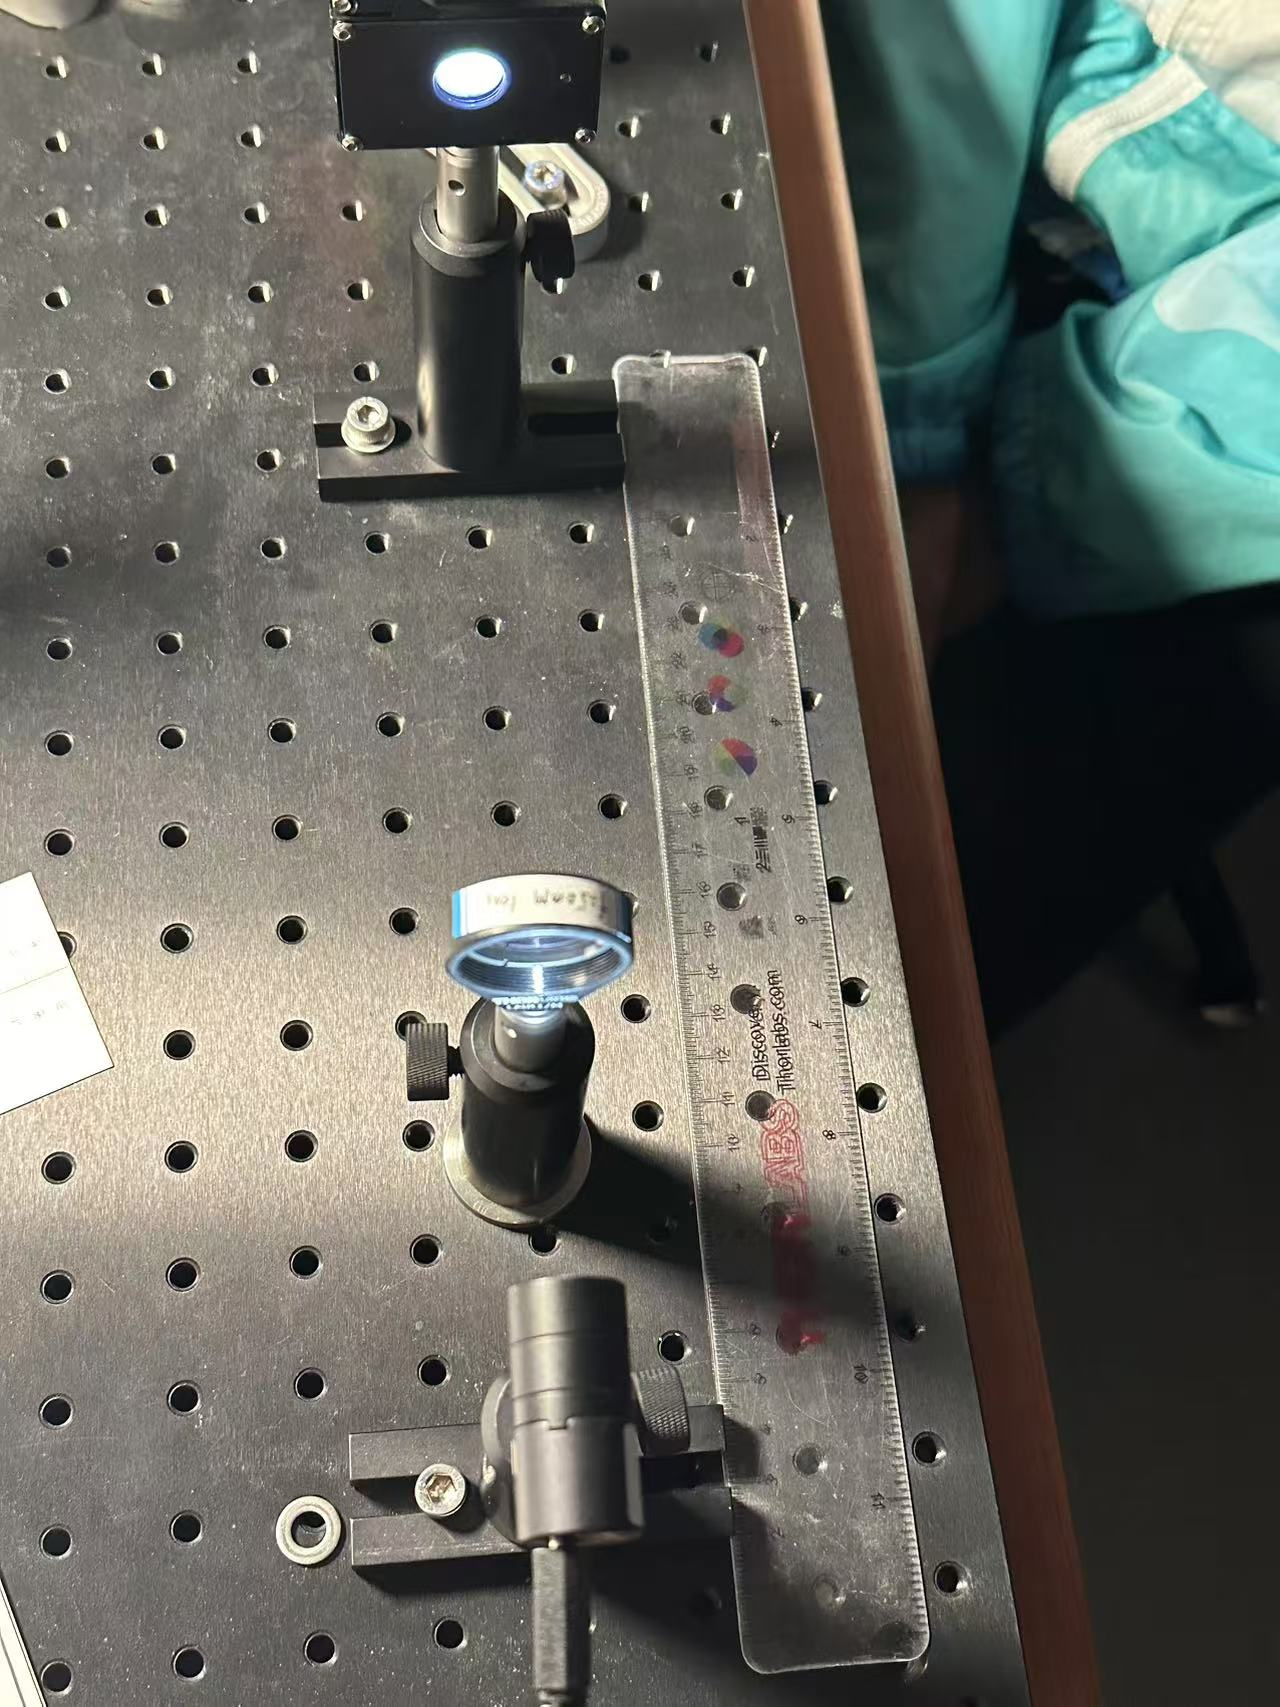
\includegraphics[width=0.2\textwidth,height=0.3\textwidth]{pictures/微信图片_20241107162037.jpg}
    \caption{LED光源安装}
\end{figure}
\section{实验步骤}

\subsection{实验一:入射狭缝宽度的影响}
1. 按照说明书组装光谱仪基本光路

2. 调节入射狭缝的宽度几乎关闭,可以看到屏幕上光强非常低

3. 慢慢打开入射狭缝,最开始可以看到像的宽度几乎不变,但是光强逐渐变强

4. 入射狭缝达到一定宽度后,再继续调节,可以看到像的宽度开始变大。这是因为狭缝的宽度已经超过了衍射极限,因此散射开始影响。

5. 完整的动态过程见视频
\subsection{实验二:LED光谱观测}
1. 将LED安装在USB供电支架上并通电。LED的光谱如图,可以看到有两个尖峰,并且在蓝色和绿色之间波长的光非常弱,几乎消失。
\begin{figure}[H]
    \centering
    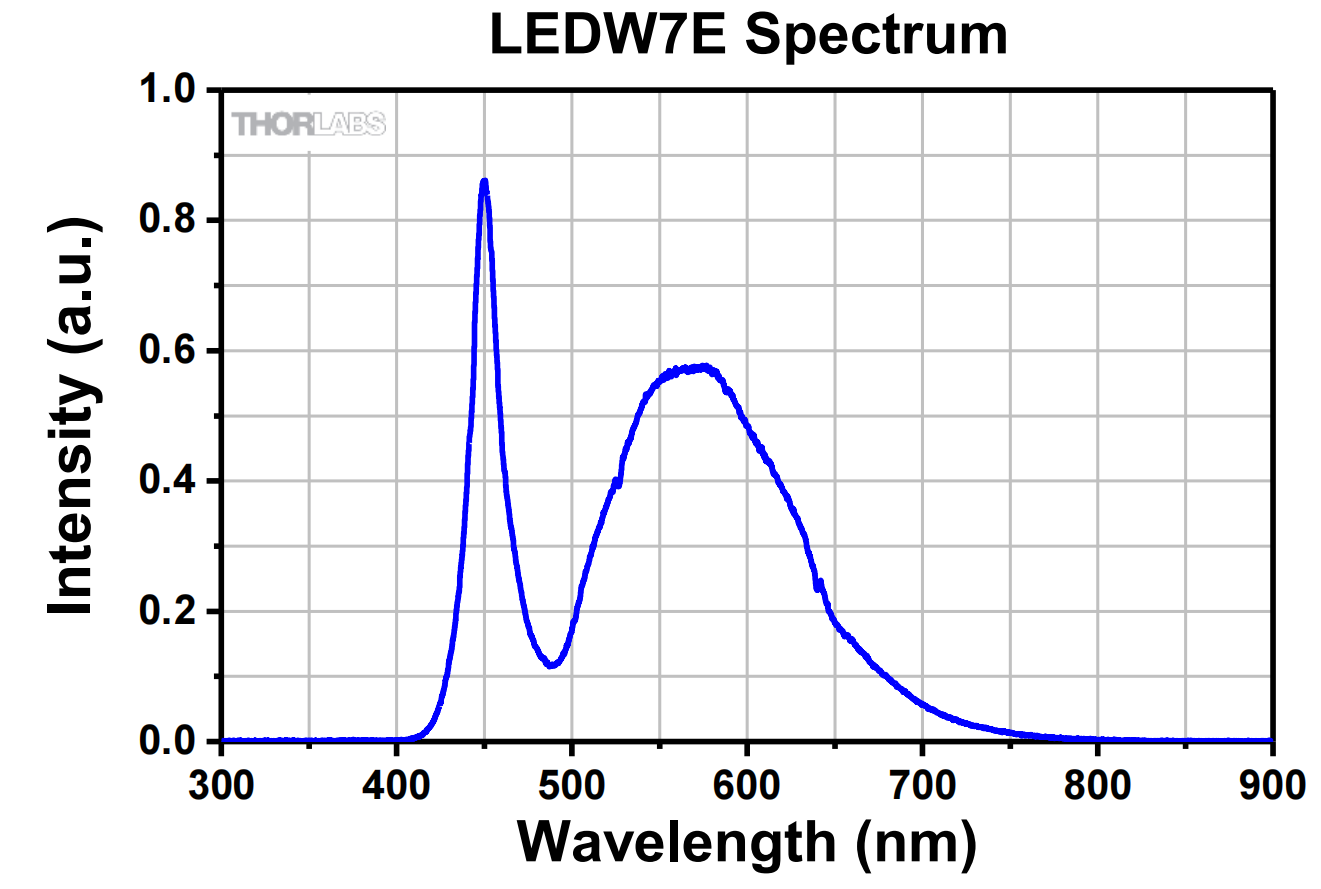
\includegraphics[width=0.4\textwidth,height=0.2\textwidth]{pictures/光谱图.png}
    \caption{LED理论光谱}
\end{figure}

2. 经过观察如图
\begin{figure}[H]
    \centering
    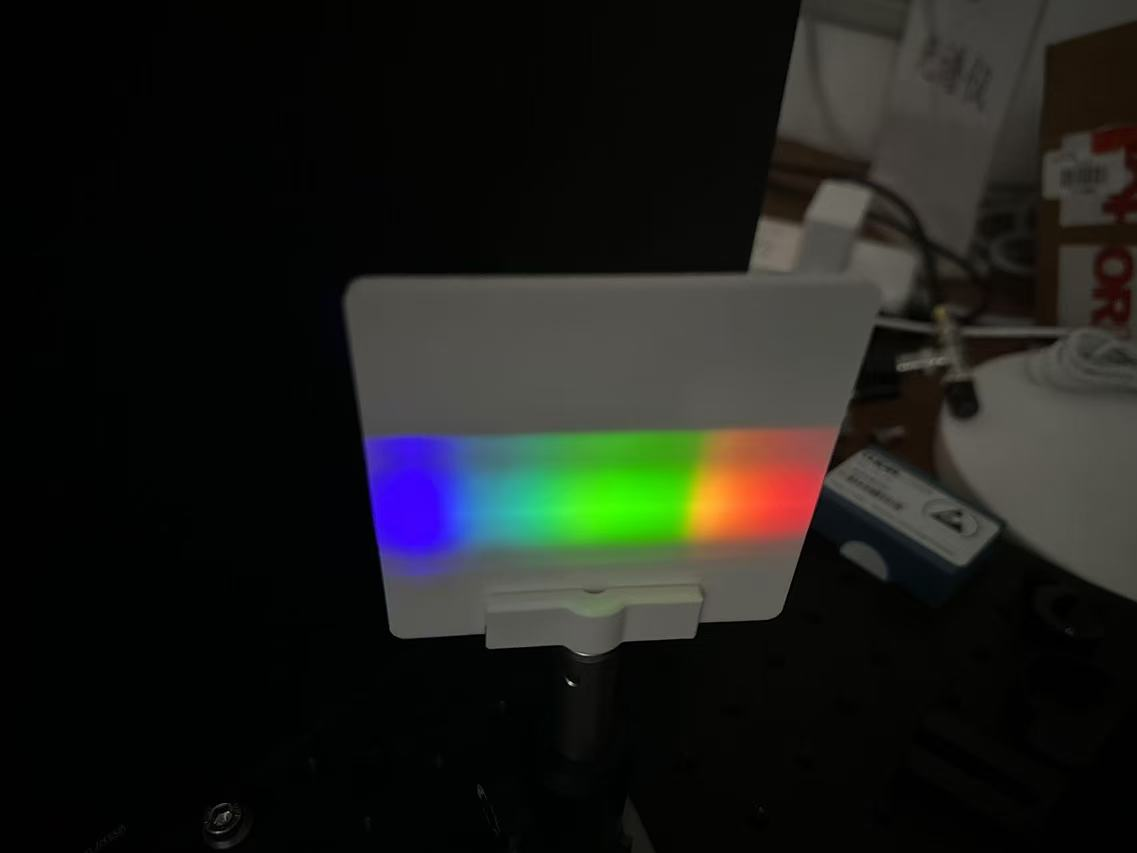
\includegraphics[width=0.4\textwidth,height=0.2\textwidth]{pictures/微信图片_20241107162045.jpg}
    \caption{LED观察光谱}
\end{figure}
与理论相符,可以看到蓝色和绿色之间的光强非常弱。

\subsection{实验三:汞光谱线波长测量}
1. 使用光栅观察汞光谱
2. 测量三条主要谱线的衍射角
3. 利用光栅方程计算波长

\section{实验思考}

\subsection{狭缝宽度的影响}
入射狭缝宽度影响光谱的分辨率和亮度。狭缝越窄,分辨率越高,但光强越弱;狭缝越宽,光强越大,但分辨率降低。这是因为狭缝宽度决定了入射光束的相干性。

\subsection{LED光谱特征}
LED发出的是连续光谱,但在特定波长范围内强度较大。这反映了LED的发光机理是由电子在半导体能带间跃迁产生的。

\subsection{光栅光谱测量}
使用光栅进行波长测量时,需要考虑衍射级数和光栅常数的影响。测量精度受到角度测量精度和光栅分辨率的限制。

\section{总结}

通过本次实验,我们:
\begin{itemize}
    \item 理解了光谱仪的基本工作原理
    \item 掌握了调节光谱仪的方法
    \item 学会了使用光栅进行波长测量
    \item 认识到了不同光源的光谱特征
\end{itemize}

实验过程中发现光路调节较为关键,需要仔细进行准直和聚焦。建议在后续实验中可以增加不同光源的对比分析,以及尝试使用棱镜进行光谱观测。

\end{document}